\documentclass[twoside,11pt]{article}
\usepackage[preprint]{jmlr2e}
\usepackage{amsmath,amssymb,bm,booktabs,array,microtype,placeins}
\graphicspath{{../figures/full/}}
\newcommand{\A}{\mathcal A}
\newcommand{\E}{\mathcal E}
\newcommand{\Pp}{\mathbb P}
\newcommand{\Ee}{\mathbb E}
\newcommand{\R}{\mathbb R}
\newcommand{\CalMultCoverage}{0.928}
\newcommand{\CalPointCoverage}{0.514}
\newcommand{\CalExactCoverage}{0.960}
\newcommand{\RareMultCoverage}{0.780}
\newcommand{\MainMultARR}{0.297}
\newcommand{\MainExactARR}{0.258}
\newcommand{\NestedReps}{200}
\newcommand{\CalibrationReps}{500}
\newcommand{\ReferenceN}{20000}
\newcommand{\MissingnessReps}{100}

\ShortHeadings{Statistical Assurance Regions}{Maale and Yi}
\firstpageno{1}
\begin{document}
\title{Statistical Assurance Regions for Predictive Models Under Joint Missingness and Distribution Shift}
\author{\name Faustus Domebale Maale \email fdmaale@aggies.ncat.edu \\
\addr Applied Science and Technology Ph.D. Program\\
College of Science and Technology\\
North Carolina A\&T State University, Greensboro, NC, USA
\AND
\name Hui Yi \email hyi@ncat.edu \\
\addr Department of Mathematics \& Statistics\\
North Carolina A\&T State University, Greensboro, NC, USA}
\editor{}
\maketitle

\begin{abstract}
A frozen predictive pipeline can satisfy a risk requirement in some deployment conditions
and fail in others. SciGuard represents this evaluation problem through a statistical assurance
region: an estimated inner subset of a prespecified environment family whose predictive risks
are bounded by a tolerance. We develop an auditable workflow using established simultaneous
inference, with finite-sample exact-binomial and bounded-loss alternatives alongside a
dependence-aware Gaussian multiplier band. We state the sampling construction that permits
shared stress transformations, distinguish uncertainty in the assurance sample from uncertainty
in simulation reference risks, and give an independent-pilot design procedure. A continuous
extension is available only with an externally justified global smoothness bound. Experiments
include nested predictive-pipeline refits, missingness-mechanism comparisons, a breast-cancer
data stress test, and computational and adverse-regime ablations. The rerun exposes limits of
Gaussian approximation: multiplier simultaneous coverage is \CalMultCoverage{} in the primary
design and \RareMultCoverage{} in a rare-event design at a nominal 0.95 level. Exact-binomial
alternatives trade efficiency for finite-sample control. A corrected MIMIC-IV temporal protocol
is implemented but has not been executed on credentialed data. The contribution is a scoped
methodological and reproducibility framework; broad deployment utility and clinical safety
are not established by the present evidence.
\end{abstract}
\begin{keywords}
deployment assurance, distribution shift, missing data, simultaneous inference, risk control
\end{keywords}

\section{Introduction}
An acceptable test-set average does not specify the conditions under which a trained model
can meet a performance requirement. A hospital, for example, may encounter changes in both
its patient population and the availability of recorded measurements. A useful validation
report would identify which explicitly modeled combinations remain supported by the data,
while distinguishing an observed low error rate from a statistically bounded risk.

We study this reporting problem for a frozen predictive pipeline. Given environments
$e_1,\ldots,e_K$, predictive risks $R_1,\ldots,R_K$, and a tolerance $\tau$, the target is
$\A_\tau=\{e_k:R_k\leq\tau\}$. A simultaneous upper band $(U_1,\ldots,U_K)$ produces
the certified inner estimate $\widehat\A_\tau=\{e_k:U_k\leq\tau\}$.
For example, upper bounds $(.07,.09,.13)$ at tolerance $.10$ certify the first two environments.
The third remains uncertified even if its point estimate is below $.10$; it has not thereby
been proven unsafe. This distinction is the basis of the statistical assurance region (SAR).

The inferential devices underlying this construction are established. Exact binomial limits,
bounded-sum inequalities, multiple testing, and Gaussian multiplier approximation already
provide ways to control joint error \citep{clopper1934,hoeffding1963,holm1979,chernozhukov2013gaussian}.
Learn then Test (LTT) can directly index its hypotheses by deployment environments
\citep{angelopoulos2025ltt}. Merely naming the resulting set does not create a new inferential
theorem. We therefore position SciGuard as an applied methodology and software workflow that
connects an explicit environment design, sampling assumptions, uncertainty accounting, and
an interpretable set-valued report.

The revision makes four substantive contributions to that workflow. First, it separates
finite-sample risk control from asymptotic dependence-aware inference and states when each
is appropriate. Second, it gives the row-level construction needed to justify reuse of
observations under multiple transformations, including corrections to a missingness generator
that previously did not implement the claimed MAR mechanism. Third, it puts nested fitted-model
experiments and reference-risk uncertainty at the center of the evaluation. Fourth, it provides
one executable notebook and shared software implementation from which all current tables and
figures are generated. An additional local MIMIC-IV protocol addresses temporal alignment,
patient separation, class imbalance, and missingness reporting, but its empirical execution
remains outstanding.

The results do not support universal use of the multiplier method. It can enlarge the certified
region when losses across environments are strongly dependent, but its simultaneous coverage
deteriorates for sparse errors in the examined finite samples. This finding motivates retaining
simple exact or bounded-loss procedures as substantive alternatives rather than weak baselines.

\section{Relationship to Existing Work}
\label{sec:related}
\paragraph{Risk control and simultaneous inference.}
Risk-controlling prediction sets and LTT provide model-agnostic calibration and testing
frameworks \citep{bates2021rcps,angelopoulos2025ltt}. In our finite-family setting, the hypotheses
$H_{0k}:R_k\geq\tau$ are an immediate LTT application. SciGuard's environment-indexed output
is an operational interpretation of this framework, not a disjoint class of guarantees.
Simultaneous confidence bands also have a substantial history beyond high-dimensional
Gaussian maxima; for example, \citet{degras2011} studies bands for functional regression.
Here the coordinates are prespecified environment-specific predictive risks. Their construction
and sampling design, rather than a new general band theorem, are the focus.

\paragraph{Prediction and adaptation under shift.}
ATC predicts target accuracy from source-calibrated confidence scores and unlabeled target
observations \citep{garg2022ood}. Its inputs and objective differ from labeled environment
certification. We therefore evaluate it using risk-prediction error, not by ranking its
``certification'' error against a formal familywise procedure. Weighted conformal prediction
addresses covariate shift using likelihood-ratio information under its stated conditions
\citep{tibshirani2019weighted}; it does not by itself give our simultaneous region over an
arbitrary family of missingness interventions. Missingness-shift adaptation changes a
predictor for target conditions \citep{zhou2023dams}. An adapted pipeline could subsequently
be frozen and assessed with the same assurance workflow.

\paragraph{Generalization bounds and robust learning.}
PAC-Bayes analysis controls the generalization of distributions over predictors using
complexity terms \citep{alquier2024}. Distributionally robust optimization changes the training
objective to improve performance over an uncertainty set \citep{duchi2021dro}. Our main route
instead conditions on a fitted pipeline and uses independent labeled assurance observations.
It makes no claim to dominate these approaches and does not transport labels to unobserved
deployment populations without additional assumptions.

\paragraph{Safe operating regions.}
\citet{dixit2025pwc} couple conformal perception calibration to a safe planner and evaluate
navigation safety. Their guarantee concerns the resulting system, whereas our risk threshold
alone says nothing about downstream control or clinical harm. \citet{torens2025odd} monitor an
operational design domain for an ML component; here uncertainty in average predictive loss
determines an inner set within an explicitly supplied family. \citet{hammar2026safe} learn a
network's safe operating region through causal observation and intervention. SciGuard's
present empirical analysis is offline and does not implement such active region expansion.
These are meaningful precedents for region-based assurance, not evidence that the term SAR
denotes a previously unstudied class of problems.

\section{Target and Sampling Design}
\label{sec:target}
Let $D_0$ include all training and design information, including preprocessing estimates,
learner randomization, a pilot sample if used, and the selected finite environment family
$\E(D_0)=\{e_1,\ldots,e_K\}$. We condition on $D_0$ unless otherwise stated. The fitted
pipeline $g$ includes imputation, transformations, prediction, and any fixed decision threshold.
For bounded loss $\ell\in[0,1]$, define
\begin{equation}
R_g(e)=\Ee_{P_e}[\ell(Y,g(X_{\mathrm{obs}},M))],\qquad
\A_\tau(g)=\{e\in\E(D_0):R_g(e)\leq\tau\}.
\label{eq:target}
\end{equation}
The law $P_e$ must be specified. Synthetic perturbation experiments establish results only
for their artificial environment laws, not automatically for a real hospital or calendar period.

\subsection{Paired stress experiments}
\begin{lemma}[Shared transformations]
\label{lem:rows}
Conditional on $D_0$, let $(Z_i,V_i)$ be i.i.d. across $i$, independent of $D_0$, and let
$h_k(\cdot;D_0)$ be fixed measurable maps into $[0,1]$. Then
$\mathbf L_i=(h_1(Z_i,V_i;D_0),\ldots,h_K(Z_i,V_i;D_0))$ are i.i.d. bounded random vectors.
No independence across coordinates is required.
\end{lemma}
\begin{proof}
For any measurable vector sets $B_1,\ldots,B_n$, the events
$\{\mathbf L_i\in B_i\}$ are measurable with respect to their respective independent
$(Z_i,V_i)$ rows, conditional on $D_0$. Their joint conditional probability factors. The
same row law and fixed maps give the same vector distribution for each $i$.
\end{proof}

Shared masks, noise, or outcome uniforms within a row are therefore compatible with
simultaneous inference. Perfectly correlated coordinates are permitted. In contrast,
normalizing missingness probabilities by the assurance-batch mean makes the transformation
depend on other rows and is not justified by Lemma~\ref{lem:rows}. Our corrected generators
use fixed population-calibrated intercepts in the simulation. Repeated patients, temporal
dependence, or cluster sampling also require an appropriate analysis rather than this i.i.d.
argument. Conditioning on training data does not remove dependence among assurance rows.

\subsection{Natural groups and independent samples}
For a master sample of independent subjects, let $G_{id}$ indicate a prespecified domain
or subgroup. With $n_d=\sum_iG_{id}$ and $\widehat p_d=n_d/n$, estimate
\begin{equation}
\widehat R_{d,m}=\frac{\sum_iG_{id}L_i^{(m)}}{n_d},\qquad
\widehat\psi_{i,d,m}=\frac{G_{id}}{\widehat p_d}
       (L_i^{(m)}-\widehat R_{d,m}).
\label{eq:group}
\end{equation}
Common row multipliers applied to these influence estimates preserve overlapping-group and
within-subject stress dependence. Fixed-dimensional asymptotic ratio inference additionally
requires positive group probabilities and nondegenerate influence variances. Small or empty
groups remain in the report and cannot certify under the prespecified minimum-size rule.
For exact binomial inference, condition on a group's membership indicators: under i.i.d.
master rows and a fixed group definition, its selected binary losses have the group-conditional
Bernoulli law. A union bound can then cover all groups and stress conditions, despite overlap.

When environments instead have genuinely independent, unequal samples, SciGuard accepts
separate loss vectors. It neither truncates all samples to their shortest length nor pairs
unrelated patients by row position. Validity remains a statement about the represented
environment populations, not unobserved sites.

\section{Risk Bounds and Set Containment}
\label{sec:inference}
\subsection{Finite-sample routes}
Let $\widehat R_k$ be the mean of $n_k$ independent bounded losses with expectation $R_k$.
For binary losses, write $S_k=n_k\widehat R_k$. The one-sided exact binomial bound is
\begin{equation}
U_k^{\mathrm{CP}}=
\begin{cases}
Q_{1-\alpha/K}\{\mathrm{Beta}(S_k+1,n_k-S_k)\},&S_k<n_k,\\
1,&S_k=n_k,
\end{cases}
\label{eq:cp}
\end{equation}
where $Q$ denotes a quantile \citep{clopper1934}. For general losses in $[0,1]$, use
\begin{equation}
U_k^{\mathrm H}=\min\left\{1,\widehat R_k+
\sqrt{\frac{\log(K/\alpha)}{2n_k}}\right\}.
\label{eq:hoeffding}
\end{equation}

\begin{proposition}[Finite-sample simultaneous assurance]
\label{prop:finite}
Conditional on the frozen design, either \eqref{eq:cp}, for Bernoulli samples, or
\eqref{eq:hoeffding}, for independent bounded samples, satisfies
\begin{equation}
\Pp\{R_k\leq U_k\ \text{for every } k\mid D_0\}\geq1-\alpha.
\label{eq:coverage}
\end{equation}
Consequently, on this same event, $\widehat\A_\tau\subseteq\A_\tau$ for every
$\tau\in[0,1]$ simultaneously. Dependence between environment samples is allowed.
\end{proposition}
\begin{proof}
An exact one-sided binomial limit fails with probability at most $\alpha/K$ in each
coordinate. For \eqref{eq:hoeffding}, the bounded-sum inequality of \citet{hoeffding1963}
gives the same marginal failure bound. The union bound yields \eqref{eq:coverage} without
requiring independence between coordinates. On that event, $U_k\leq\tau$ implies
$R_k\leq U_k\leq\tau$ for every coordinate and every threshold.
\end{proof}

These are standard constructions, stated here to make the software guarantee explicit.
For example, $S_k=0$ gives $U_k^{\mathrm{CP}}=1-(\alpha/K)^{1/n_k}$, a positive uncertainty
bound despite no observed errors. Exact Holm uses $p_k=\Pp\{\mathrm{Bin}(n_k,\tau)\leq S_k\}$
and the step-down rule of \citet{holm1979}. These are valid lower-tail tests of
$H_{0k}:R_k\geq\tau$ and yield finite-sample familywise containment at that fixed tolerance.
The method is an environment-indexed LTT instantiation; it need not supply a full upper band.

\subsection{Dependence-aware multiplier route}
For paired rows, define $\widehat\sigma_k^2=n^{-1}\sum_i(L_{ik}-\widehat R_k)^2$ and
\begin{equation}
T^*=\max_k\left\{-\frac{1}{\sqrt n\widehat\sigma_k}
                   \sum_{i=1}^n\xi_i(L_{ik}-\widehat R_k)\right\},
\quad \xi_i\stackrel{\mathrm{iid}}\sim N(0,1).
\label{eq:multiplier}
\end{equation}
Let $c^*_{1-\alpha}$ be its conditional quantile. The upper band is
\begin{equation}
U_k^{\mathrm M}=\min\{1,\widehat R_k+
             c^*_{1-\alpha}\widehat\sigma_k/\sqrt n\}.
\label{eq:multupper}
\end{equation}
Software enlarges negative simulated critical values to zero and assigns bound 1 to
empirically constant columns. This avoids invalid studentization; it is not a general repair
for rare-event approximation error.

\begin{proposition}[Fixed-family asymptotic justification]
\label{prop:mult}
Under Lemma~\ref{lem:rows}, for fixed $K$ and positive population coordinate variances,
the ideal conditional quantile in \eqref{eq:multiplier} yields
$\liminf_{n\to\infty}\Pp(R_k\leq U_k^{\mathrm M}\text{ for all }k\mid D_0)\geq1-\alpha$.
For an empirical bootstrap quantile, the statement also requires the number of draws to
increase sufficiently for quantile estimation error to vanish.
\end{proposition}
\begin{proof}
The multivariate central limit theorem applies to the independent bounded loss vectors.
The sample covariance converges entrywise to the population covariance and each sample
standard deviation converges to a positive constant. Conditional on the data, the vector
in \eqref{eq:multiplier} before taking its maximum is exactly Gaussian with the empirical
standardized covariance. Its distribution therefore converges to the same Gaussian limit
as the standardized mean errors. The maximum of finitely many Gaussian coordinates with
nonzero marginal variance has a continuous distribution, even if the covariance is singular.
Quantile consistency and the continuous mapping argument give asymptotic coverage.
The set-containment implication then follows as in Proposition~\ref{prop:finite}.
\end{proof}

For increasing $K$, the high-dimensional results of \citet{chernozhukov2013gaussian}
provide sufficient regimes for bounded coordinates with uniformly positive variances;
a familiar conservative regime is $\log^7(Kn)/n\to0$ under the associated regularity constants.
Lemma~\ref{lem:rows} establishes the relevant independent-vector construction; bounded losses
and a uniform variance lower bound supply its basic moment conditions. This rate is not a
practical sample-size prescription. Later refinements improve Gaussian and bootstrap
approximation rates \citep{cckk2022}; we do not assert their sharpest rates or optimality for
the present grouped and stressed-data implementation. The experiments assess finite-sample
behavior directly and show that the assumptions can be practically uninformative for rare errors.

\begin{figure}[t]
\centering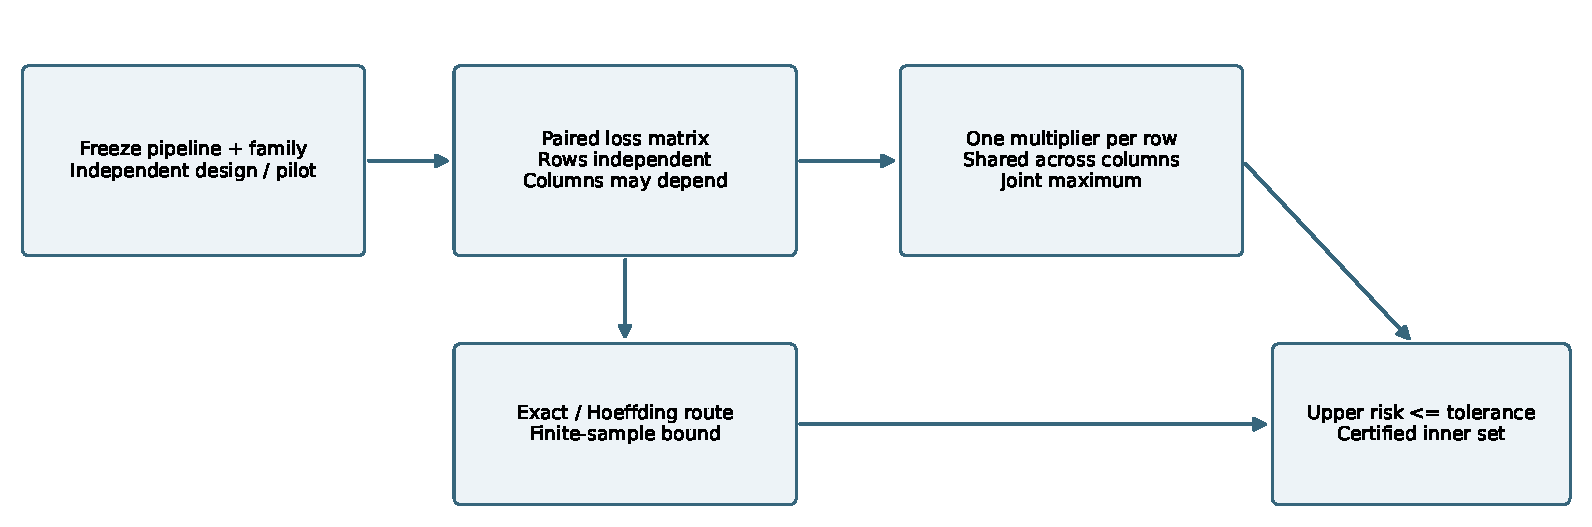
\includegraphics[width=\linewidth]{workflow.pdf}
\caption{The workflow separates the sampling design from the choice of inferential bound.
The multiplier route shares one random weight across all losses in a row. Exact and
bounded-loss alternatives reach the same set-valued output with different guarantees.}
\label{fig:workflow}
\end{figure}

\subsection{Conditioning, tuning, and repeated use}
If a finite-sample statement holds conditional on every admissible training/design realization,
averaging over $D_0$ preserves its error bound. Nested refits illustrate variation across fitted
pipelines; they do not transform an asymptotic method into a finite-sample theorem.
Proposition~\ref{prop:finite} also clarifies a useful distinction: a fixed risk band supports
all tolerances simultaneously, including a threshold inspected afterward. That mathematical
fact does not justify retroactively defining an operationally meaningful risk requirement.
Changing models, losses, families, or choosing the most favorable unadjusted method after
assurance is different and requires protection over the enlarged selection problem.

Repeated 95\% checks are not a time-uniform 95\% statement. A simple conservative extension
uses fresh assurance data at round $t$, conditions on the past, and applies a finite-sample
procedure at $\alpha_t=\alpha/[t(t+1)]$. Since $\sum_{t\geq1}\alpha_t=\alpha$, a union bound
controls any erroneous certification over all rounds. This standard spending argument does
not supply efficient adaptive or optimal sequential region learning.

\section{Environment Design and Continuous Regions}
\label{sec:design}
The environment family is a scientific input. Begin with a specified loss and decision
threshold, define interpretable axes and externally motivated ranges, and distinguish changes
to the population from changes to measurement or observation. A transformation of one labeled
sample is not evidence that an intended real deployment law is represented. Omitted axes
remain outside the scope of the report.

Our independent-pilot procedure starts with a candidate grid, retains points near a
pilot-estimated boundary together with coordinate extremes, and freezes that selected finite
family before examining an independent assurance sample. Conditional on the pilot, the exact
binomial construction applies without selective-inference machinery. Alternatively, one may
first construct a valid band on an entire fixed superset and report a subset of it. Reusing the
same outcomes to invent new environments and applying an unadjusted band only afterward is
not justified by either argument.

For planning, \eqref{eq:hoeffding} has additive width at most $\epsilon$ when
$n\geq\log(K/\alpha)/(2\epsilon^2)$. This bound is conservative and controls band width,
not the probability of certifying a cell with a particular true risk. Pilot simulations can
estimate recall for plausible risk margins, but they cannot establish external validity.

Suppose a compact continuous family has a scientifically justified global bound
$|R(e)-R(e')|\leq L_Rd(e,e')$. Define
\begin{equation}
U^{\mathrm{cont}}(e)=\min\left\{1,\min_{k\leq K}[U_k+L_Rd(e,e_k)]\right\}.
\label{eq:continuous}
\end{equation}
On the grid-coverage event, $R(e)\leq R(e_k)+L_Rd(e,e_k)\leq U_k+L_Rd(e,e_k)$ for
every $k$, so \eqref{eq:continuous} covers the risk everywhere. Thresholding it gives a
continuous inner region. This is a standard smoothness consequence of simultaneous inference.

The largest observed slope on a finite grid is not a valid global upper bound on $L_R$.
An independent pilot removes selection bias but cannot exclude unobserved rapid variation
between design points without structural assumptions. If an externally justified random
$\widehat L_R$ bounds the global constant with failure probability $\delta$, the combined
error budget is at most $\alpha+\delta$. Without such a bound, finite-grid certification
and explicitly assumption-dependent smoothness sensitivity are the defensible outputs.

\section{Experimental Design and Evaluation}
\label{sec:experiments}
All reported results are generated by the revised shared implementation, with seed 20260927.
They supersede the historical CSVs retained under \texttt{archive/pre\_revision/}. Models,
designs, and inferential settings are fixed in code; outcomes are not filtered to match earlier
published-looking numbers. The full profile and smoke profile write separate directories.
Tables and numerical macros are exported from full-run CSVs with a hash-based provenance record.

With known risk vector $R$, containment is
$C=\mathbb I\{\widehat\A_\tau\subseteq\A_\tau\}$,
ARR is $|\widehat\A_\tau\cap\A_\tau|/|\A_\tau|$, and UCP is
$|\widehat\A_\tau\setminus\A_\tau|/|\widehat\A_\tau|$. We set UCP to zero for an empty
certified set and leave ARR undefined when the true safe set is empty. Counts accompany these
metrics. A high containment frequency can be vacuous when almost nothing is certified, and it
does not imply that a full risk band covers at its advertised confidence level.
Wilson intervals describe Monte Carlo uncertainty in binary coverage/containment indicators;
mean recalls and paired differences have replication-level Monte Carlo standard errors (MCSEs).

\subsection{Nested fitted-pipeline study}
\label{sec:nested}
The central predictive-pipeline experiment uses \NestedReps{} independent refits. Each generates
1,200 training rows, 400 source-calibration rows for ATC, 1,000 assurance rows, and
\ReferenceN{} separate reference rows. Ten Gaussian covariates have AR(1) covariance with
parameter $.35$. Outcomes follow
\begin{equation}
\Pp(Y=1\mid X)=\operatorname{expit}\left[1.5\{.75X_0-.65X_1+.45X_2
+ .55X_0X_1-.35X_2^2+.20X_3\}\right].
\label{eq:dgp}
\end{equation}
A fixed normalized direction $d\propto(.8,-.6,.4,.2,0,\ldots,0)$ induces mean shift
$s\Sigma^{1/2}d$, using the Cholesky factor. The grid has
$m\in\{0,.1,.2,.3\}$ and $s\in\{0,.15,.30,.45\}$, with $\tau=.35$.
Feature $X_0$ remains observed for comparability with the MAR study; severity $m$ is the
missingness rate among the other nine features. Imputation uses training means.
The two pipelines are standardized logistic regression and histogram gradient boosting
(60 boosting iterations, 15 maximum leaves, learning rate $.08$). The same base rows,
label uniforms, and missingness randomness are used across models and environments.

The independent reference mean $\widetilde R_k$ is not called an oracle truth. Simultaneous
two-sided exact binomial intervals $[a_k,b_k]$ allocate total error $.01$ over both models'
reference risks within each refit. Define confirmed-safe cells by $b_k\leq\tau$,
confirmed-unsafe cells by $a_k>\tau$, and all others as ambiguous. Then
\begin{equation}
\begin{aligned}
C^- &=\mathbb I\{\text{all certified cells are confirmed safe}\},\\
C^+ &=\mathbb I\{\text{no certified cell is confirmed unsafe}\}.
\end{aligned}
\label{eq:reference}
\end{equation}
satisfy $C^-\leq C\leq C^+$ on that reference-coverage event. The means of these endpoints
are reported as a reference bracket, not as confidence limits for a coverage probability.
Point-reference containment and ARR remain labeled as such. The reference interval budget
is per refit; it is not a joint $.99$ guarantee over all refits.

\begin{table}[t]
\centering\small\setlength{\tabcolsep}{4pt}
\caption{Nested refits. LR denotes logistic regression and HGB histogram gradient boosting.
The reference bracket averages \eqref{eq:reference}; it captures reference-risk ambiguity,
not Monte Carlo uncertainty in a population coverage probability. ARR uses reference means.}
\label{tab:nested}\begin{tabular}{llrrr}
\toprule
Model & Method & Reference containment [95\% CI] & ARR & Reference bracket \\
\midrule
LR & Bonferroni normal & 1.000 [0.981, 1.000] & 0.167 & [0.960, 1.000] \\
LR & Multiplier & 1.000 [0.981, 1.000] & 0.237 & [0.940, 1.000] \\
LR & Bonferroni exact & 1.000 [0.981, 1.000] & 0.139 & [0.970, 1.000] \\
LR & Hoeffding & 1.000 [0.981, 1.000] & 0.047 & [0.995, 1.000] \\
LR & Exact Holm & 1.000 [0.981, 1.000] & 0.167 & [0.955, 1.000] \\
HGB & Bonferroni normal & 1.000 [0.981, 1.000] & 0.669 & [1.000, 1.000] \\
HGB & Multiplier & 1.000 [0.981, 1.000] & 0.735 & [1.000, 1.000] \\
HGB & Bonferroni exact & 1.000 [0.981, 1.000] & 0.631 & [1.000, 1.000] \\
HGB & Hoeffding & 1.000 [0.981, 1.000] & 0.395 & [1.000, 1.000] \\
HGB & Exact Holm & 1.000 [0.981, 1.000] & 0.732 & [1.000, 1.000] \\
\bottomrule
\end{tabular}

\end{table}

Table~\ref{tab:nested} gives point-reference containment 1.000 for all methods, which must
not be read as proof of perfect containment. Logistic-regression cells near the boundary
remain ambiguous under the reference intervals; the reference bracket is wider for the
multiplier procedure. HGB has no ambiguous reference cells in these runs, making its favorable
recall a result for this particular fitted-model regime rather than evidence about difficult
near-boundary clinical cases. The relative advantage over exact Holm is also model-dependent:
the two methods have nearly equal HGB recall. Figure~\ref{fig:nested} makes these differences
visible without assigning ATC a certification interpretation.

\begin{figure}[t]
\centering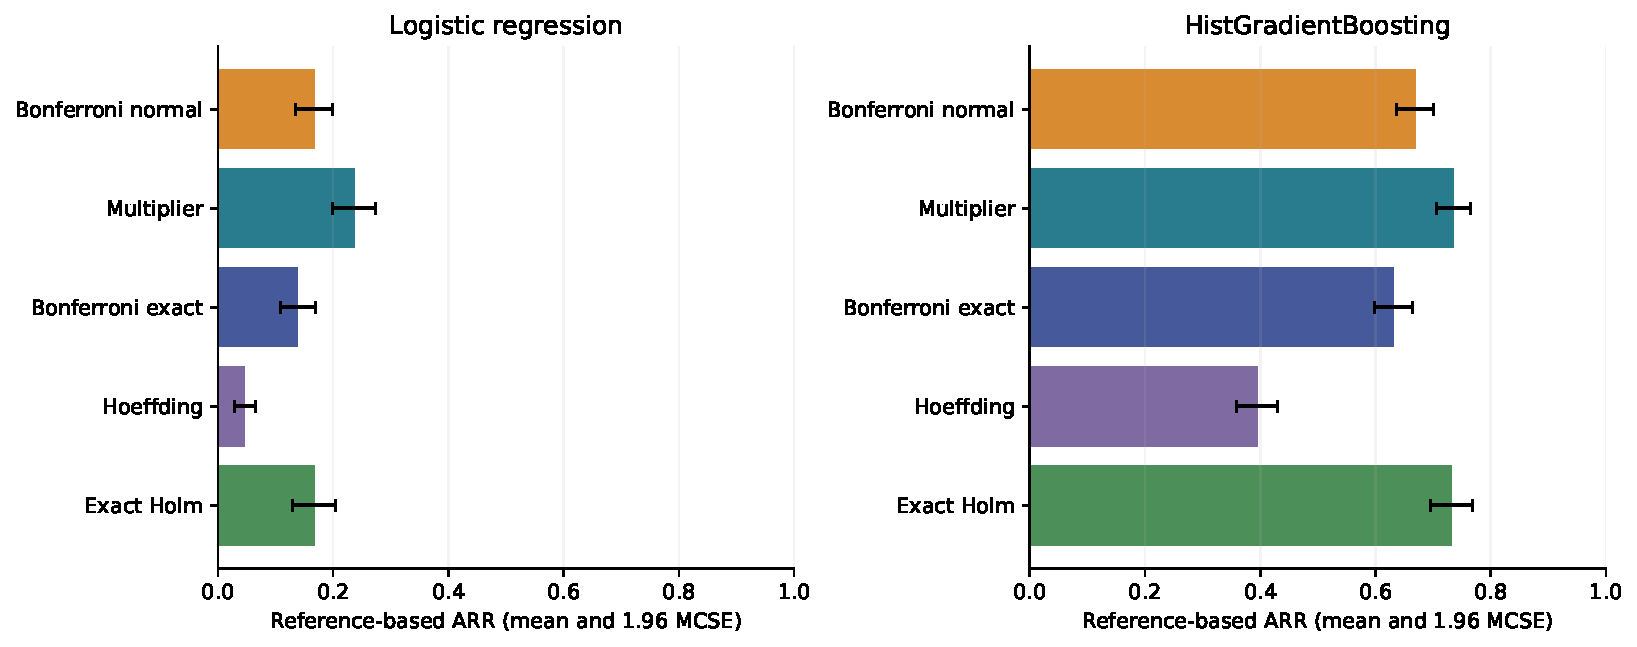
\includegraphics[width=\linewidth]{nested.pdf}
\caption{Reference-based recall across nested refits. Bars are means; error bars are 1.96
MCSE. These error bars describe Monte Carlo variation, not uncertainty in the reference risks.}
\label{fig:nested}
\end{figure}

ATC uses maximum class probability and a source-calibrated strict threshold, with tied scores
handled jointly. Table~\ref{tab:atc} reports its risk-prediction MAE, signed bias, and RMSE
against the independent reference means. No target labels enter its risk predictions, whereas
the certification methods use labeled assurance losses. This is a descriptive neighboring
task, not a head-to-head comparison of equal guarantees.
\begin{table}[t]
\centering\small
\caption{ATC-MC performance prediction, averaged over nested refits.}
\label{tab:atc}\begin{tabular}{lrrr}
\toprule
Model & MAE & Bias & RMSE \\
\midrule
Logistic regression & 0.031 & -0.012 & 0.033 \\
HistGradientBoosting & 0.030 & -0.014 & 0.032 \\
\bottomrule
\end{tabular}

\end{table}

\subsection{Missingness-mechanism study}
\label{sec:missing}
Across \MissingnessReps{} logistic-regression refits, we compare MCAR, MAR, MNAR, and
structured missingness with the same training and evaluation design. MAR depends only on
always-observed $X_0$; MNAR depends on the latent value of the feature being hidden. Logistic
intercepts solve a population Gaussian expectation equation for the target marginal missingness,
using 64-node Gaussian quadrature. They are fixed before evaluation and are not normalized
using assurance rows. Structured failure makes features 1--3 missing together, with every
eligible feature retaining marginal severity $m$. The original cyclic driver scheme could
hide its own conditioning variables and was not a valid general MAR implementation.

Reference intervals allocate error $.01$ over all four mechanisms within each refit.
Table~\ref{tab:missing} shows that the reference uncertainty can matter even when every
point-reference containment indicator equals one. In particular, ambiguous cells reduce the
MCAR multiplier lower endpoint. These results concern the chosen parameterizations; they do
not imply that MNAR is generally easier or safer than MCAR. Realized missingness fractions
and all exact-baseline comparisons are retained in the current-run CSVs.
\begin{table}[t]
\centering\small\setlength{\tabcolsep}{4pt}
\caption{Multiplier results for missingness mechanisms. Ambiguous cells are averaged over
the 16 environments per refit. All metrics use the corrected mechanism definitions.}
\label{tab:missing}\begin{tabular}{lrrrr}
\toprule
Mechanism & Reference containment & Reference bracket & ARR & Ambiguous cells \\
\midrule
MCAR & 1.000 [0.963, 1.000] & [0.940, 1.000] & 0.211 & 1.83 \\
MAR & 1.000 [0.963, 1.000] & [0.990, 1.000] & 0.249 & 0.28 \\
MNAR & 1.000 [0.963, 1.000] & [1.000, 1.000] & 0.303 & 0.00 \\
Structured & 1.000 [0.963, 1.000] & [0.930, 1.000] & 0.232 & 0.98 \\
\bottomrule
\end{tabular}

\end{table}
\begin{figure}[t]
\centering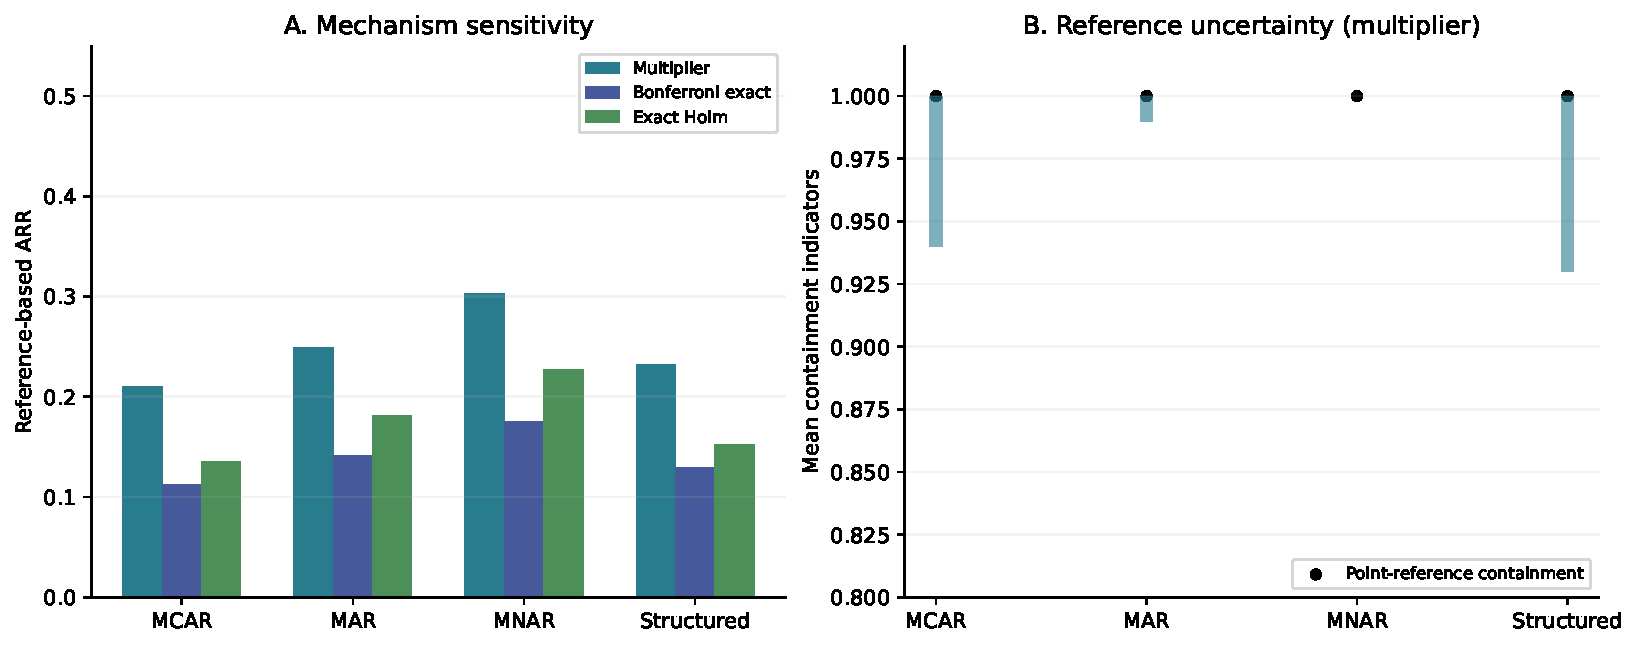
\includegraphics[width=\linewidth]{missingness.pdf}
\caption{Mechanism sensitivity and the effect of reference-risk uncertainty. Vertical segments
in panel B span mean lower/upper containment indicators; they are not confidence intervals.}
\label{fig:missing}
\end{figure}

\subsection{Calibration with exactly known risks}
\label{sec:calibration}
To isolate inference, a Gaussian copula generates binary losses with the 25 marginal risks
stored in the supplied simulation surface, $n=1000$, latent correlation $.55$, and $\tau=.34$.
We run \CalibrationReps{} replications and 2,000 multiplier draws per replication. This is a
calibration experiment, not a fitted-pipeline deployment study. All methods receive the same
loss matrix in each replication.

\begin{table}[t]
\centering\small\setlength{\tabcolsep}{4pt}
\caption{Primary calibration study. Coverage is simultaneous risk-band coverage. Holm supplies
fixed-tolerance tests rather than a risk band, so its coverage entry is inapplicable.}
\label{tab:cal}\begin{tabular}{lrrrr}
\toprule
Method & Coverage [95\% CI] & Containment [95\% CI] & ARR & UCP \\
\midrule
Pointwise normal & 0.514 [0.470, 0.558] & 0.958 [0.937, 0.972] & 0.522 & 0.0042 \\
Bonferroni normal & 0.938 [0.913, 0.956] & 0.998 [0.989, 1.000] & 0.282 & 0.0002 \\
Multiplier & 0.928 [0.902, 0.948] & 0.998 [0.989, 1.000] & 0.297 & 0.0002 \\
Bonferroni exact & 0.960 [0.939, 0.974] & 0.998 [0.989, 1.000] & 0.258 & 0.0002 \\
Hoeffding & 1.000 [0.992, 1.000] & 1.000 [0.992, 1.000] & 0.138 & 0.0000 \\
Exact Holm & -- & 0.998 [0.989, 1.000] & 0.270 & 0.0002 \\
\bottomrule
\end{tabular}

\end{table}

Pointwise normal intervals attain only \CalPointCoverage{} simultaneous coverage. The multiplier
band attains \CalMultCoverage{}, compared with \CalExactCoverage{} for exact Bonferroni
(Table~\ref{tab:cal}). The multiplier's mean ARR is \MainMultARR{}, compared with
\MainExactARR{} for exact Bonferroni. This efficiency difference accompanies different
finite-sample validity: the multiplier is not a finite-sample replacement for exact inference.
Its primary coverage estimate lies below $.95$; the Monte Carlo interval describes the
precision of that finding and does not verify a universal nominal guarantee.

\begin{figure}[t]
\centering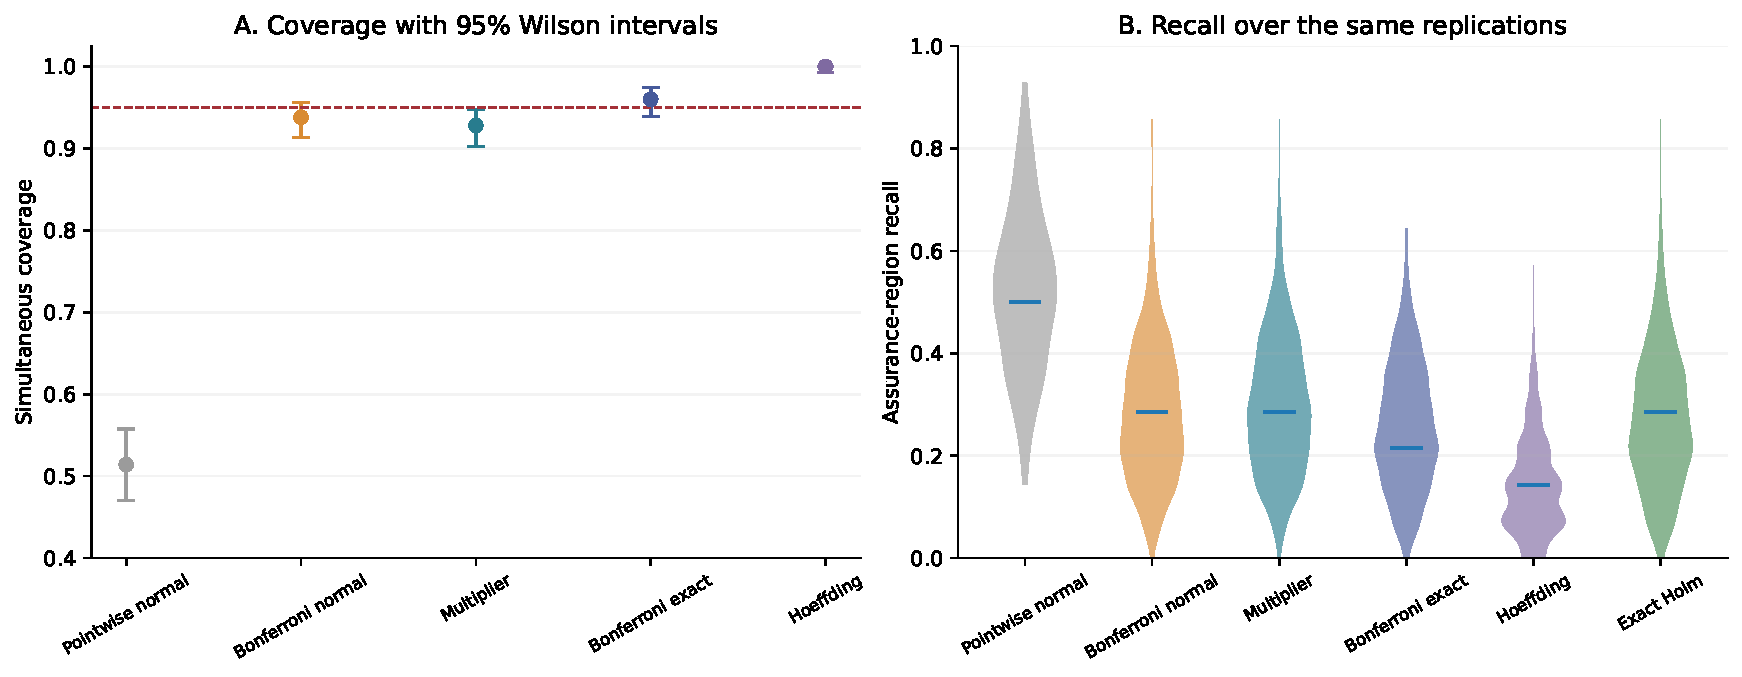
\includegraphics[width=\linewidth]{calibration.pdf}
\caption{Simultaneous coverage and the recall distribution over primary replications. The
dashed line is the nominal coverage target; higher recall alone does not establish validity.}
\label{fig:cal}
\end{figure}

\subsection{Dependence, sample size, and adverse regimes}
\label{sec:stress}
The sensitivity study uses 300 replications per setting, varying $n\in\{500,1000,5000\}$
at latent correlation $.55$ and correlation $\rho\in\{.10,.55,.90\}$ at $n=1000$.
Table~\ref{tab:gains} reports paired recall gains, not differences between independently
simulated studies. Against normal Bonferroni the gain is negligible at low correlation and
larger at high correlation. Comparison with exact Holm is necessary: exploiting dependence
is not the only way to reduce multiplicity conservatism.
\begin{figure}[t]
\centering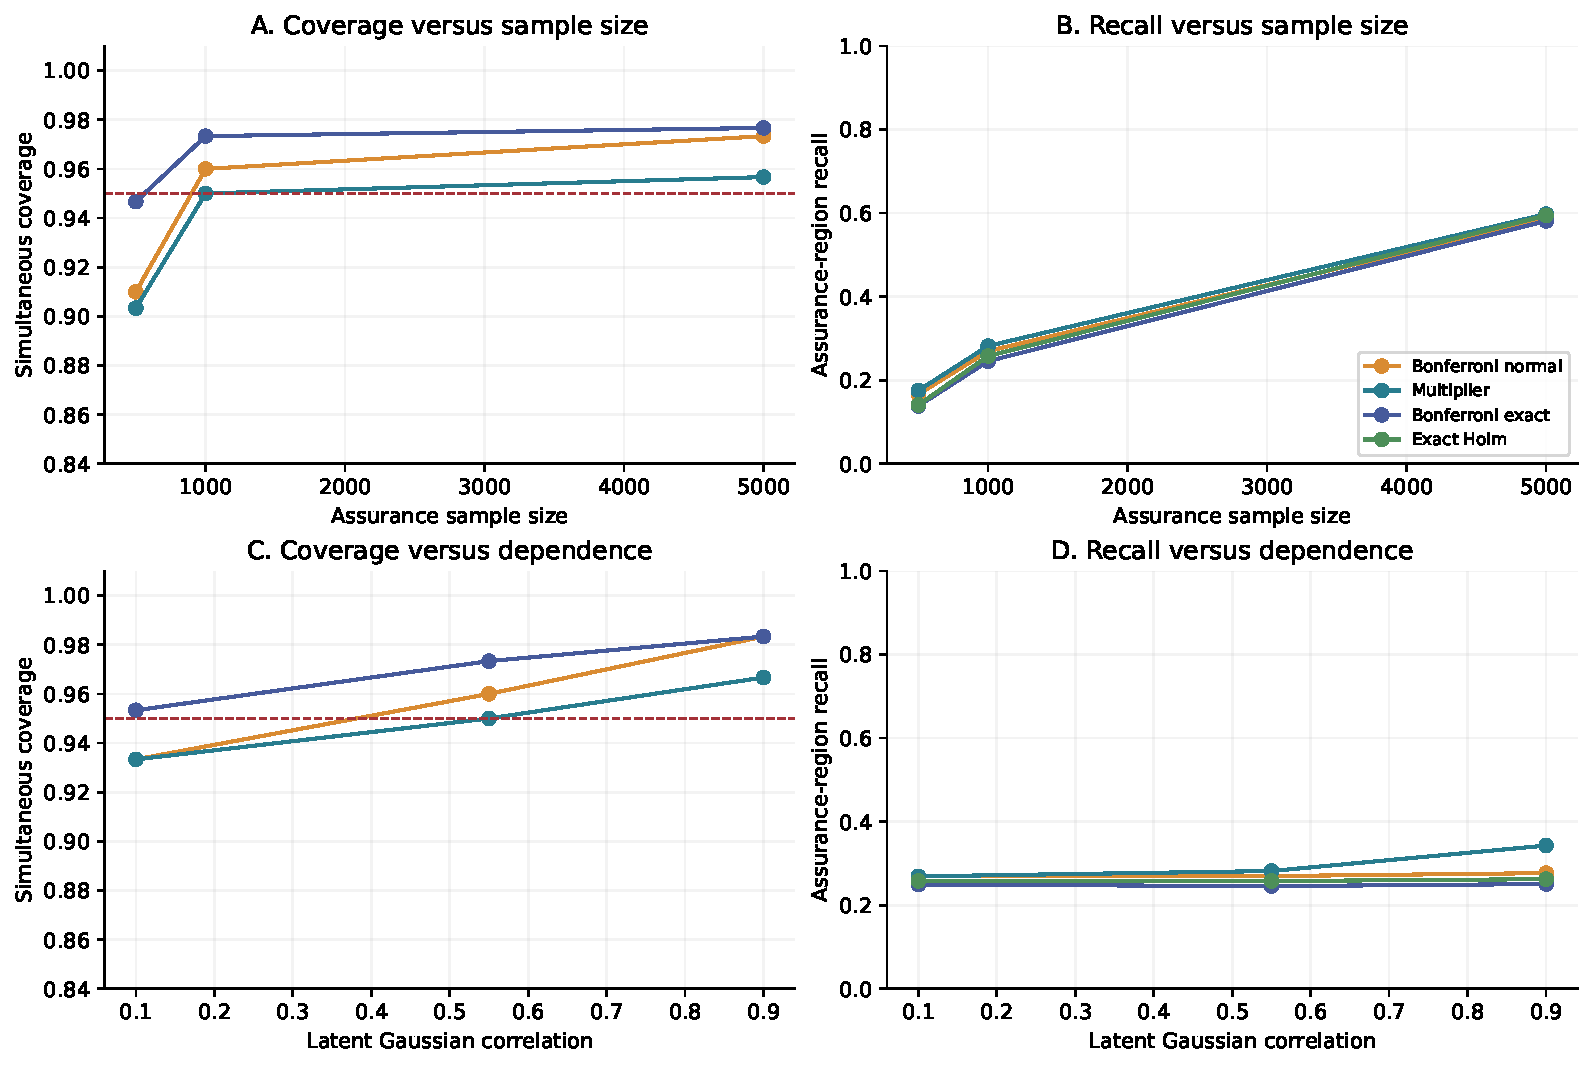
\includegraphics[width=.96\linewidth]{sensitivity.pdf}
\caption{Coverage and recall sensitivity. Latent Gaussian correlation is a generator parameter,
not the observed binary-loss correlation. Holm is omitted from risk-band coverage panels.}
\label{fig:sensitivity}
\end{figure}

Three additional 200-replication settings challenge the main result: independent Beta losses
with concentration four and known means from the main surface; binary risks equally spaced
from $.002$ to $.08$ at $n=500$, $K=25$, and $\tau=.035$; and a $K=125$ binary family at
$n=1000$ formed by repeating the main risk values with new copula-specific noise. The last
setting enlarges the number of hypotheses, not the dimensionality of continuous deployment
geometry. Losses remain bounded; no robustness claim is made for unbounded heavy tails or
adversarially selected environments.

The rare-event multiplier coverage is \RareMultCoverage{} (Table~\ref{tab:stress}). Refusing
to certify zero-variance columns does not prevent this failure in low-count, nonconstant
columns. Exact binomial methods remain applicable, and Hoeffding can be very conservative.
These adverse results provide a practical reason to prefer a finite-sample route when such
control is required. Selecting whichever unadjusted bound yields the most certificates after
seeing assurance losses is not a valid remedy.
\begin{table}[t]
\centering\small\setlength{\tabcolsep}{4pt}
\caption{Adverse-regime results. Exact binomial bounds are not applicable to continuous losses.}
\label{tab:stress}\begin{tabular}{llrrr}
\toprule
Scenario & Method & Coverage [95\% CI] & Containment & ARR \\
\midrule
Continuous bounded & Bonferroni normal & 0.925 [0.880, 0.954] & 1.000 & 0.469 \\
Continuous bounded & Multiplier & 0.925 [0.880, 0.954] & 1.000 & 0.470 \\
Continuous bounded & Hoeffding & 1.000 [0.981, 1.000] & 1.000 & 0.008 \\
Rare binary & Bonferroni normal & 0.780 [0.718, 0.832] & 0.995 & 0.455 \\
Rare binary & Multiplier & 0.780 [0.718, 0.832] & 0.990 & 0.502 \\
Rare binary & Bonferroni exact & 0.995 [0.972, 0.999] & 1.000 & 0.379 \\
Rare binary & Hoeffding & 1.000 [0.981, 1.000] & 1.000 & 0.000 \\
Larger binary family & Bonferroni normal & 0.945 [0.904, 0.969] & 0.995 & 0.208 \\
Larger binary family & Multiplier & 0.910 [0.862, 0.942] & 0.990 & 0.232 \\
Larger binary family & Bonferroni exact & 0.960 [0.923, 0.980] & 0.995 & 0.188 \\
Larger binary family & Hoeffding & 0.995 [0.972, 0.999] & 1.000 & 0.088 \\
\bottomrule
\end{tabular}

\end{table}
\begin{figure}[t]
\centering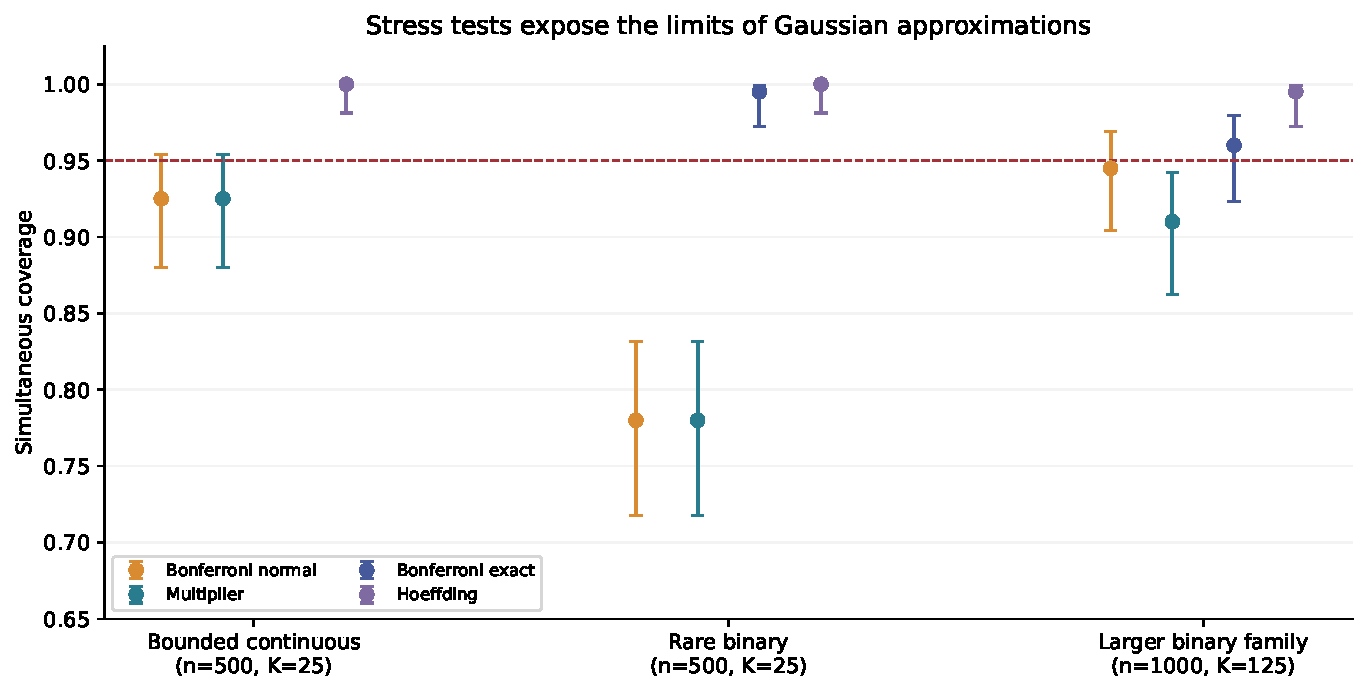
\includegraphics[width=.95\linewidth]{stress.pdf}
\caption{Coverage failures in adverse regimes, with 95\% Wilson intervals.}
\label{fig:stress}
\end{figure}

\subsection{Continuous example and independent pilot}
The illustrative surface $R(m,s)=.24+.12m+.10s+.05ms$ on
$[0,.4]\times[0,.6]$ has a valid Euclidean Lipschitz bound
$L_R=\sqrt{.15^2+.12^2}$. We use a $5\times5$ assurance grid, $\tau=.32$, 200 replications,
and an $81\times81$ mesh to compute numerical recall and containment diagnostics.
Table~\ref{tab:continuous} distinguishes grid coverage from mesh containment. The analytical
argument for \eqref{eq:continuous}, not the dense mesh, supplies coverage over every point
when the grid band and the global bound are valid. Separate exports evaluate sensitivity to
half and twice the analytic bound; the half-bound is not asserted valid.
\begin{table}[t]
\centering\small
\caption{Continuous example. Mesh recall is an equal-grid-point area approximation.}
\label{tab:continuous}\begin{tabular}{lrrrr}
\toprule
Method & Grid coverage & Mesh containment & Mesh recall & Mesh UCP \\
\midrule
Multiplier & 0.940 & 0.975 & 0.460 & 0.0004 \\
Bonferroni exact & 0.965 & 0.980 & 0.404 & 0.0001 \\
Hoeffding & 1.000 & 1.000 & 0.185 & 0.0000 \\
\bottomrule
\end{tabular}

\end{table}
\begin{figure}[t]
\centering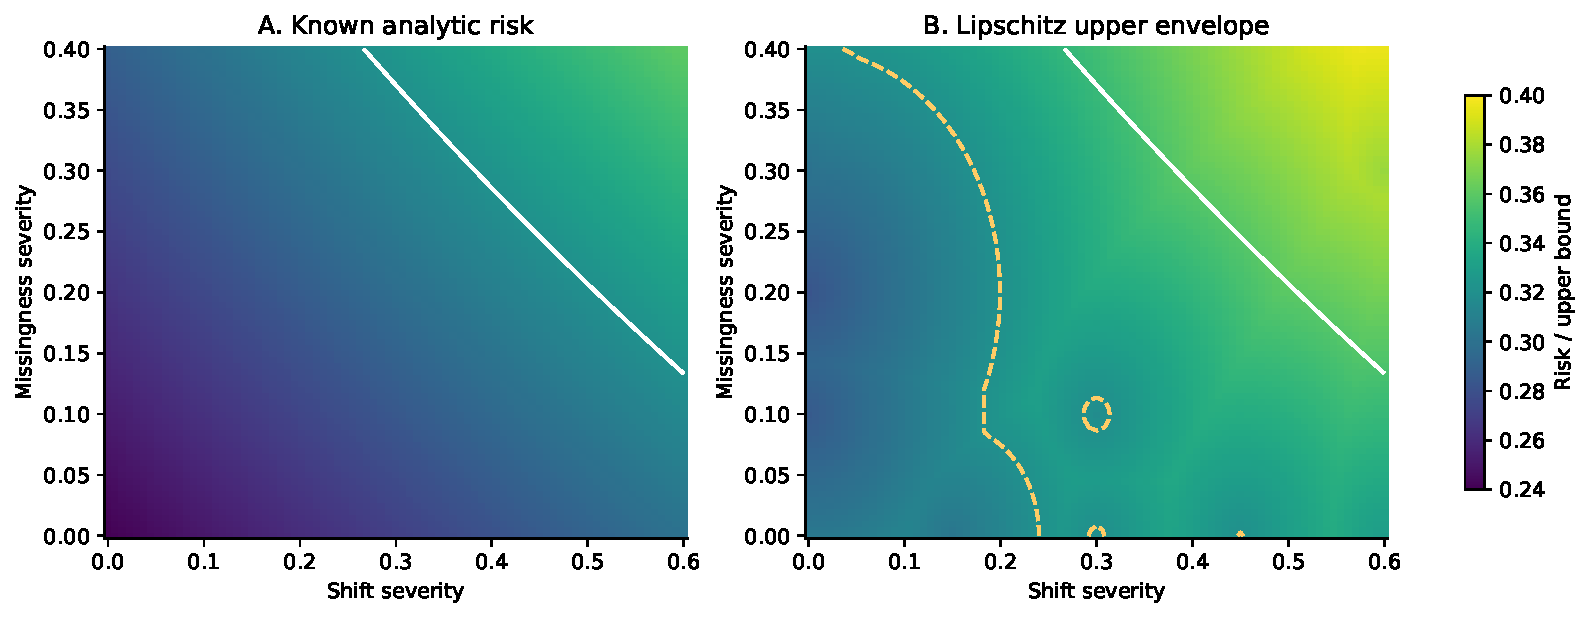
\includegraphics[width=\linewidth]{continuous.pdf}
\caption{One fixed replication of the continuous example. White denotes the true tolerance
boundary; the dashed gold curve denotes the displayed surface's tolerance contour.}
\label{fig:continuous}
\end{figure}

The pilot example starts with an $11\times11$ candidate grid on the same rectangle.
Using 300 independent pilot rows, it retains points whose pilot risks are within $.015$ of
$.32$ and coordinate extrema, then certifies the selected family on new assurance rows with
exact Bonferroni. Two hundred replications and a sample-size planning table are exported.
This demonstrates a valid split-sample workflow; it does not establish an optimal adaptive
grid or certification of all unselected points.

\section{Wisconsin Diagnostic Breast Cancer Stress Test}
\label{sec:wdbc}
The supplied WDBC data contain 569 observations. A fixed stratified 65/35 split produces
369 training rows and 200 assurance rows. The frozen models are standardized logistic
regression, an Extra Trees ensemble with 500 trees, and histogram gradient boosting.
Training means impute missing values; Gaussian feature noise is scaled by training standard
deviations. One noise matrix and one uniform missingness matrix are shared across stress
conditions and models. The primary family uses
$m\in\{0,.05,.10,.20,.30,.40\}$ and $s\in\{0,.10,.20,.30,.40,.50\}$.
The multiplier uses 5,000 draws. Table~\ref{tab:wdbc} includes exact procedures so that
Gaussian and finite-sample answers are not conflated in this small sample.

\begin{table}[t]
\centering\small
\caption{WDBC results for separate model-specific 36-environment families. The nominal
observed risk is descriptive. Counts at two tolerances do not establish clinical safety.}
\label{tab:wdbc}\begin{tabular}{llrrr}
\toprule
Model & Method & Nominal risk & Certified $\tau=.08$ & Certified $\tau=.10$ \\
\midrule
LR & Multiplier & 0.010 & 23/36 & 30/36 \\
LR & Bonferroni normal & 0.010 & 20/36 & 29/36 \\
LR & Bonferroni exact & 0.010 & 15/36 & 23/36 \\
LR & Exact Holm & 0.010 & 15/36 & 27/36 \\
Extra Trees & Multiplier & 0.035 & 9/36 & 19/36 \\
Extra Trees & Bonferroni normal & 0.035 & 2/36 & 17/36 \\
Extra Trees & Bonferroni exact & 0.035 & 0/36 & 9/36 \\
Extra Trees & Exact Holm & 0.035 & 0/36 & 9/36 \\
HGB & Multiplier & 0.045 & 2/36 & 14/36 \\
HGB & Bonferroni normal & 0.045 & 0/36 & 12/36 \\
HGB & Bonferroni exact & 0.045 & 0/36 & 2/36 \\
HGB & Exact Holm & 0.045 & 0/36 & 2/36 \\
\bottomrule
\end{tabular}

\end{table}
\begin{figure}[t]
\centering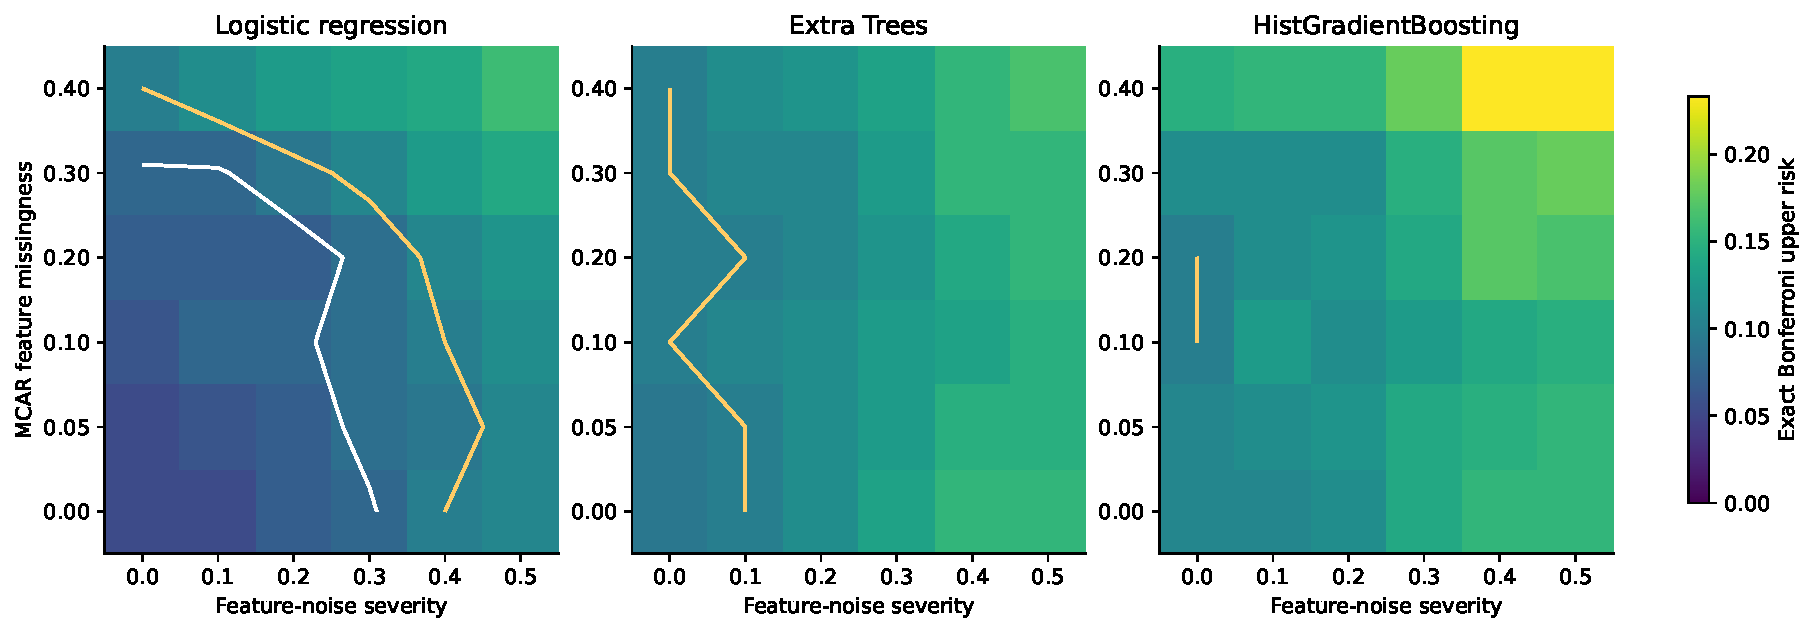
\includegraphics[width=\linewidth]{wdbc.pdf}
\caption{Exact Bonferroni risk surfaces for the three models. White and gold contours, where
present, mark tolerances $.08$ and $.10$. Absence of a contour can mean no grid crossing.}
\label{fig:wdbc}
\end{figure}

Logistic regression has the lowest nominal observed error in this split, but counts depend
strongly on the method and tolerance. These are separate model-specific simultaneous
statements: choosing a model by comparing these bands does not confer joint model-selection
coverage. The tolerances are illustrative, not medical standards. WDBC perturbations are
synthetic and do not represent observed temporal or inter-hospital shifts; its single split
cannot estimate the true deployment safe set, ARR, or a coverage probability.

Equally spaced $4\times4$, $6\times6$, and $10\times10$ logistic grids span the same
rectangle. Their results appear in Table~\ref{tab:grid}. The primary 36-cell grid is nonuniform
in missingness and is not identical to the equally spaced $6\times6$ grid. Certified grid
fractions cannot be interpreted as continuous areas without an additional design measure
or smoothness argument. A grid is not selected retrospectively for the largest certificate.

\section{MIMIC-IV: Implemented Protocol and Remaining Evidence}
\label{sec:mimic}
\textbf{No MIMIC-IV results are claimed in this revision.} The supplied archive contains
neither credentialed MIMIC tables nor a completed benchmark output. The earlier primary
notebook stopped at its MIMIC section with a missing-file error. We provide a corrected local
execution path and validate its mechanics using synthetic table fixtures; that test is not
clinical evidence. A genuine naturally shifted evaluation remains necessary to address the
central empirical limitation of the present manuscript.

The protocol targets in-hospital mortality for the first eligible adult admission per patient,
using admission-table variables only. It excludes identifiers, outcome flags, discharge or
death times, and length of stay from predictors. Age top-coding is retained explicitly.
The field-availability audit for the intended admission-time decision must still be completed
on the actual data; a demographic/admission model is a limited baseline, not a comprehensive
clinical prediction system.

MIMIC-IV shifts dates separately for each patient. Its documentation instructs users to align
stays to the anchor year rather than treat a patient's \texttt{anchor\_year\_group} as the period
of every admission \citep{mimic31,johnson2023mimic}. The loader adds the shifted admission-year
offset to both group endpoints and, by default, pads the approximate interval by one year
for year-boundary ambiguity. This padding is an analysis choice, not an official exact-date
guarantee. Intervals are restricted to the declared dataset coverage. Source intervals must
end by the prespecified cutoff and deployment intervals begin afterward; overlapping
intervals are excluded. Deployment groups are approximate admission intervals, which may
overlap one another in calendar time, rather than exact years or distinct hospitals.

The example configuration describes v3.1, with source ending by 2016 and subsequent
deployment intervals. Users must supply the actual version, scientifically justified tolerance,
and rationale before running. The former illustrative $.35$ mortality-error tolerance is not
carried forward as a meaningful clinical requirement. Unweighted logistic regression and
histogram gradient boosting are fitted on source patients, with a source holdout kept separate.
An always-survive classifier is included. All models, groups, and missingness conditions form
one family for the clinical certification comparison, avoiding unadjusted selection across models.

The protocol reports mortality prevalence, sensitivity, specificity, balanced accuracy, AUROC,
and AUPRC, because low misclassification risk alone can be misleading for rare outcomes.
These diagnostics do not inherit the 0--1-risk guarantee. Native feature missingness is
reported separately from synthetic MCAR additions and total missingness. The grouped
influence construction \eqref{eq:group}, exact group-conditional binomial bounds, Hoeffding,
and Holm accommodate unequal group sizes without fabricating row alignment. Small groups
are retained as uncertified. One admission per patient addresses repeated-patient rows but
does not establish independence across time or hospital processes.

Only aggregate tables, the frozen configuration, and source-file hashes are exported by the
local protocol. No patient-level cohort or fitted model is included in this revision. Completing
the external evaluation requires inspecting actual cohort flow, temporal support, native
missingness, label and feature timing, prevalence, trivial-baseline performance, and effective
sample sizes before any benchmark result is promoted into the manuscript.

\section{Practical Interpretation and Limitations}
\label{sec:discussion}
\paragraph{Choosing a method.}
Use an exact binary-loss procedure when finite-sample control is central and the independent
sampling model is defensible; use a bounded-loss inequality for other bounded losses when
conservatism is acceptable. A multiplier band can be useful when the family is strongly
dependent and validation supports the approximation, but the rare-event experiment shows
that sample size alone is not a sufficient diagnostic. Compare paired recall gains with exact
Holm as well as normal Bonferroni, and inspect validity at the same time. The method should
be fixed in advance or multiplicity should cover any subsequent method selection.

\paragraph{What is established.}
We give a coherent assurance target, transparent sampling and inference contracts, a
standard finite-sample route, a justified fixed-family multiplier construction, corrected
mechanism simulations, explicit reference uncertainty, and reproducible comparisons.
The framework accepts any frozen pipeline yielding bounded losses, but the experiments
cover a small number of tabular model classes. Interface generality is not empirical evidence
for arbitrary neural architectures or deployment systems.

\paragraph{What remains open.}
The inferential components do not constitute a new optimality theorem. No minimax recovery
rate, general safe exploration guarantee, or efficient time-uniform adaptive grid is proved.
The continuous extension depends on external smoothness. Unknown shifts and causal
transportability remain outside the certificate. Unbounded heavy-tailed losses and adversarial
adaptation are not studied. Reference-risk uncertainty persists near the tolerance even with
20,000 rows. The primary simulation deliberately calibrates inference, and WDBC remains
small and semisynthetic. The unexecuted MIMIC protocol cannot fill the missing natural-shift
evidence. These limitations prevent a claim of general deployment readiness.

\section{Conclusion}
SciGuard connects a prespecified deployment family to an explicit, auditable set-valued
risk report. Established finite-sample and bootstrap tools provide different routes to that
report, with different assumptions and efficiency. The revised experiments show both the
benefit of accounting for dependence and consequential Gaussian-approximation failures.
The appropriate conclusion is a scoped applied framework with reproducible evidence and
an implementable external-validation protocol. Stronger claims require completed natural-shift
evaluation and, if theoretical novelty is the objective, results beyond the standard
simultaneous-inference and smoothness arguments used here.

\section*{Data and Code Availability}
The source code, reproducibility notebook, configuration files, aggregate experimental outputs,
figures, tests, and manuscript materials are publicly available at
\url{https://github.com/dfmaale/sciguard-sar}. The exact \texttt{v1.0.0} release used for this
study is permanently archived at Zenodo: \url{https://doi.org/10.5281/zenodo.23228566}.
MIMIC-IV is a credentialed dataset and is therefore not redistributed with the repository.
Eligible users may obtain access directly from PhysioNet and reproduce the analysis using the
supplied protocol and configuration files. Only aggregate MIMIC-IV outputs are included in the
public archive.

\appendix
\section{Additional Tables}
\begin{table}[ht]
\centering\small
\caption{Paired mean ARR gain of multiplier over each comparator. MCSE uses paired
replication differences. These efficiency comparisons must be read with coverage results.}
\label{tab:gains}\begin{tabular}{rrlrr}
\toprule
$n$ & $\rho$ & Comparator & Paired ARR gain & MCSE \\
\midrule
500 & 0.55 & Bonferroni normal & 0.009 & 0.0016 \\
1000 & 0.10 & Bonferroni normal & -0.000 & 0.0008 \\
1000 & 0.55 & Bonferroni normal & 0.012 & 0.0016 \\
1000 & 0.90 & Bonferroni normal & 0.066 & 0.0038 \\
5000 & 0.55 & Bonferroni normal & 0.012 & 0.0017 \\
500 & 0.55 & Bonferroni exact & 0.037 & 0.0029 \\
1000 & 0.10 & Bonferroni exact & 0.020 & 0.0020 \\
1000 & 0.55 & Bonferroni exact & 0.036 & 0.0029 \\
1000 & 0.90 & Bonferroni exact & 0.092 & 0.0041 \\
5000 & 0.55 & Bonferroni exact & 0.016 & 0.0019 \\
500 & 0.55 & Exact Holm & 0.035 & 0.0029 \\
1000 & 0.10 & Exact Holm & 0.011 & 0.0016 \\
1000 & 0.55 & Exact Holm & 0.024 & 0.0023 \\
1000 & 0.90 & Exact Holm & 0.080 & 0.0041 \\
5000 & 0.55 & Exact Holm & 0.003 & 0.0010 \\
\bottomrule
\end{tabular}

\end{table}
\begin{table}[ht]
\centering\small
\caption{Equally spaced WDBC logistic-regression grid ablation.}
\label{tab:grid}\begin{tabular}{llrrr}
\toprule
Grid & Method & $K$ & Certified $\tau=.08$ & Fraction \\
\midrule
4x4 & Multiplier & 16 & 10 & 0.625 \\
4x4 & Bonferroni exact & 16 & 7 & 0.438 \\
6x6 & Multiplier & 36 & 23 & 0.639 \\
6x6 & Bonferroni exact & 36 & 11 & 0.306 \\
10x10 & Multiplier & 100 & 69 & 0.690 \\
10x10 & Bonferroni exact & 100 & 23 & 0.230 \\
\bottomrule
\end{tabular}

\end{table}
\FloatBarrier

\section{Computational Cost and Bootstrap Variability}
The direct multiplier sampler requires $O(BnK)$ operations. Sampling from its conditional
Gaussian covariance instead costs $O(nK^2+K^3+BK^2)$ and stores a $K\times K$ covariance;
it can be advantageous for moderate $K$. The code chooses that route when $K\leq\min(n,2000)$
and retains a chunked row-multiplier route otherwise. Conditional distributional equivalence
is tested with identical-column and independent-column constructions. Numerical agreement
between samplers does not verify frequentist coverage.

The timing study holds the loss matrix fixed and repeats each bootstrap size under 25
independent seeds. Table~\ref{tab:runtime} separates the number of observations, environments,
and bootstrap draws. Timings depend on machine and numerical libraries and exclude loss
generation/model fitting. The critical-value MCSE is the standard error of its mean across
seeds, not a guaranteed quantile error bound. Per-seed critical values and certified counts
are also exported so bootstrap variability is inspectable directly.
\begin{table}[ht]
\centering\small
\caption{Conditional-covariance multiplier timing and variability.}
\label{tab:runtime}\begin{tabular}{lrrrrr}
\toprule
$n$ & $K$ & $B$ & Critical mean & Critical MCSE & Mean seconds \\
\midrule
500 & 25 & 200 & 2.819 & 0.0188 & 0.0015 \\
500 & 25 & 1000 & 2.795 & 0.0085 & 0.0021 \\
500 & 25 & 5000 & 2.796 & 0.0052 & 0.0055 \\
1000 & 25 & 200 & 2.806 & 0.0289 & 0.0018 \\
1000 & 25 & 1000 & 2.793 & 0.0089 & 0.0025 \\
1000 & 25 & 5000 & 2.794 & 0.0037 & 0.0055 \\
1000 & 125 & 200 & 3.257 & 0.0227 & 0.0096 \\
1000 & 125 & 1000 & 3.213 & 0.0097 & 0.0152 \\
1000 & 125 & 5000 & 3.210 & 0.0035 & 0.0322 \\
\bottomrule
\end{tabular}

\end{table}

\section{Planning and Verification}
\begin{table}[ht]
\centering\small
\caption{Conservative assurance-sample planning for a Hoeffding additive width at most the
stated margin, with $\alpha=.05$. This is not a guarantee of a particular recall.}
\label{tab:planning}\begin{tabular}{lrr}
\toprule
$K$ & Margin & Sufficient $n$ \\
\midrule
25 & 0.02 & 7769 \\
25 & 0.05 & 1243 \\
25 & 0.10 & 311 \\
100 & 0.02 & 9502 \\
100 & 0.05 & 1521 \\
100 & 0.10 & 381 \\
500 & 0.02 & 11513 \\
500 & 0.05 & 1843 \\
500 & 0.10 & 461 \\
\bottomrule
\end{tabular}

\end{table}
Tests cover finite-sample binomial error by enumerating possible counts, the zero-error
bound, empirical degeneracy, duplicated columns, covariance/row multiplier equivalence,
unequal samples, overlapping and empty groups, reference boundaries, MAR row locality,
ATC ties, and admission-aligned MIMIC cohort construction. The synthetic MIMIC fixture exercises
the complete local pipeline and aggregate-output schema. It is discarded after testing and
is never treated as a benchmark dataset. The canonical notebook imports these same functions,
records configuration and package versions, and generates its manuscript inputs from the
completed full run rather than hard-coded target values.

\bibliography{references}
\end{document}
